%%%%%%%%%%%%%%%%%%%%%%%%%%%%%%%%%%%%%%%%%
% Short Sectioned Assignment LaTeX Template Version 1.0 (5/5/12)
% This template has been downloaded from: http://www.LaTeXTemplates.com
% Original author:  Frits Wenneker (http://www.howtotex.com)
% License: CC BY-NC-SA 3.0 (http://creativecommons.org/licenses/by-nc-sa/3.0/)
%%%%%%%%%%%%%%%%%%%%%%%%%%%%%%%%%%%%%%%%%

%----------------------------------------------------------------------------------------
%	PACKAGES AND OTHER DOCUMENT CONFIGURATIONS
%----------------------------------------------------------------------------------------

\documentclass[paper=a4, fontsize=11pt]{scrartcl} % A4 paper and 11pt font size

% ---- Entrada y salida de texto -----

\usepackage[T1]{fontenc} % Use 8-bit encoding that has 256 glyphs
\usepackage[utf8]{inputenc}

% ---- Idioma --------

\usepackage[spanish, es-tabla]{babel} % Selecciona el español para palabras introducidas automáticamente, p.ej. "septiembre" en la fecha y especifica que se use la palabra Tabla en vez de Cuadro

% ---- Otros paquetes ----

\usepackage{amsmath,amsfonts,amsthm} % Math packages
\usepackage{graphics,graphicx, floatrow} %para incluir imágenes y notas en las imágenes
\usepackage{graphics,graphicx, float} %para incluir imágenes y colocarlas
\usepackage{hyperref} % url in references

% Para hacer tablas comlejas
\usepackage{multirow}
\usepackage{threeparttable}

\usepackage{fancyhdr} % Custom headers and footers
\pagestyle{fancyplain} % Makes all pages in the document conform to the custom headers and footers
\fancyhead{} % No page header - if you want one, create it in the same way as the footers below
\fancyfoot[L]{} % Empty left footer
\fancyfoot[C]{} % Empty center footer
\fancyfoot[R]{\thepage} % Page numbering for right footer
\renewcommand{\headrulewidth}{0pt} % Remove header underlines
\renewcommand{\footrulewidth}{0pt} % Remove footer underlines
\setlength{\headheight}{13.6pt} % Customize the height of the header

\numberwithin{equation}{section} % Number equations within sections (i.e. 1.1, 1.2, 2.1, 2.2 instead of 1, 2, 3, 4)
\numberwithin{figure}{section} % Number figures within sections (i.e. 1.1, 1.2, 2.1, 2.2 instead of 1, 2, 3, 4)
\numberwithin{table}{section} % Number tables within sections (i.e. 1.1, 1.2, 2.1, 2.2 instead of 1, 2, 3, 4)

\setlength\parindent{0pt} % Removes all indentation from paragraphs - comment this line for an assignment with lots of text

\newcommand{\horrule}[1]{\rule{\linewidth}{#1}} % Create horizontal rule command with 1 argument of height

\usepackage{textcomp}
\usepackage{hyperref}

%----------------------------------------------------------------------------------------
%	DATOS
%----------------------------------------------------------------------------------------

\newcommand{\myName}{Francisco Javier Bolívar Lupiáñez}
\newcommand{\myDegree}{Máster en Ingeniería Informática}
\newcommand{\myFaculty}{E. T. S. de Ingenierías Informática y de Telecomunicación}
\newcommand{\myDepartment}{Ciencias de la Computación e Inteligencia Artificial}
\newcommand{\myUniversity}{\protect{Universidad de Granada}}
\newcommand{\myLocation}{Granada}
\newcommand{\myTime}{\today}
\newcommand{\myTitle}{Práctica 2}
\newcommand{\mySubtitle}{Uso de contenedores (Docker)}
\newcommand{\mySubject}{Cloud Computing: Servicios y Aplicaciones}
\newcommand{\myYear}{2016-2017}

%----------------------------------------------------------------------------------------
%	PORTADA
%----------------------------------------------------------------------------------------


\title{	
	\normalfont \normalsize 
	\textsc{\textbf{\mySubject \space (\myYear)} \\ \myDepartment} \\[20pt] % Your university, school and/or department name(s)
	\textsc{\myDegree \\[10pt] \myFaculty \\ \myUniversity} \\[25pt]
	\horrule{0.5pt} \\[0.4cm] % Thin top horizontal rule
	\huge \myTitle: \mySubtitle \\ % The assignment title
	\horrule{2pt} \\[0.5cm] % Thick bottom horizontal rule
	\normalfont \normalsize
}

\author{\myName} % Nombre y apellidos

\date{\myTime} % Incluye la fecha actual
%----------------------------------------------------------------------------------------
%	INDICE
%----------------------------------------------------------------------------------------

\begin{document}
	
\definecolor{light-gray}{gray}{0.95}
	
\lstset {
	basicstyle=\scriptsize,
	frame=single,
	backgroundcolor=\color{grey}
}

\lstdefinestyle{PHP}{
	frame=single,
	numbers=left,
	language=PHP,
	basicstyle=\footnotesize,
	keywordstyle=\bfseries,
	commentstyle=\itshape,
	identifierstyle=\bfseries,
}
	
\setcounter{page}{0}

\maketitle % Muestra el Título
\thispagestyle{empty}

\newpage %inserta un salto de página

\tableofcontents % para generar el índice de contenidos

%\listoffigures

\newpage

%----------------------------------------------------------------------------------------
%	DOCUMENTO
%----------------------------------------------------------------------------------------

\section{Introducción}

El objetivo de esta práctica es familiarizarse con el uso de una plataforma PaaS y desarrollar habilidades de despliegue de contenedores y configurar aplicaciones sencillas en los mismos.
\\ \\
Para ello el alumno deberá realizar las tareas que se describen a continuación y entregar documentación describiendo con el mayor detalle posible todas las actividades realizadas.
\\ \\
Dentro de la plataforma de prácticas habilitada para la asignatura, DOCKER, accesible a través de hadoop.ugr.es (vía ssh), cada alumno deberá:

\begin{itemize}
	\item Crear un contenedor (A) con APACHE, SSL y PHP5.
	\begin{itemize}
		\item ¿Cuál es el puerto SSL?
		\item ¿Cómo redirigir el puerto SSL a vuestro puerto asignado?
	\end{itemize}
	\item Crear un contenedor (B) con MySQL.
	\item Crear una página en el servidor web (A) que se conecte al servicio MySQL en el contenedor (B).
	\item Duplicar los contenedores A y B y discutir o mostrar qué pasaría si uno de ellos cayese.
	\item Desplegar un servicio OwnCloud o NewCloud en otro contenedor (o eliminar alguno de los ya utilizados) y chequear su correcto funcionamiento almacenando archivos.
	\item Elaborar un breve documento detallando todo el trabajo realizado.
\end{itemize}

\section{Descripción de la aplicación web}

Se ha desarrollado una aplicación web lo más simple posible, pues lo verdaderamente importante en esta práctica era el despliegue y conexión de máquinas virtuales.
\\ \\
La aplicación web solo permite consultar y añadir estrellas que podemos observar en el cielo nocturno almacenando su nombre y su distancia en años luz. Por tanto solo cuenta con una tabla: \texttt{Star(id, name, distance)}.
\\ \\
Como se ha mencionado anteriormente, y se puede intuir por lo que se ha instalado en cada máquina virtual, se utiliza SQL para la base de datos, PHP en el \textit{back-end} de la aplicación y HTML y CSS en el \textit{front-end} usando una plantilla de Bootstrap.

\section{Contenedores para la web}

Para la aplicación web, como ya se hizo en la práctica anterior, se hará uso de Apache, PHP y MySQL (MariaDB).
\\ \\
Para ello se crearán dos contenedores, uno con MariaDB y otro con Apache y PHP5 \cite{DockerPHPMySQL} \cite{DockerMariaDB}.
\\ \\
Lo primero que hay que hacer es descargar los contenedores que se utilizarán:

\begin{lstlisting}
docker pull nimmis/apache-php5
docker pull mariadb
\end{lstlisting}

Una vez descargados, se podrán crear los dos contenedores, enlazando el de la base de datos al de la web:

\begin{lstlisting}
docker run -d -p PORT:3306 --name fblupi-db -e MYSQL_ROOT_PASSWORD=PWD mariadb
docker run -d -p PORT:80 --name fblupi-web --link fblupi-db:db nimmis/apache-php5 
\end{lstlisting}

Si accedemos al servidor web podremos ver la página de inicio de Apache, ahora hay que instalar tanto la base de datos como la aplicación.

\subsection{Base de datos}

Accedemos a una terminal del contenedor:

\begin{lstlisting}
docker exec -i -t fblupi-db bash
\end{lstlisting}

Lo primero que habrá que hacer es instalar git para poder descargar el script de creación de la base de datos:

\begin{lstlisting}
apt-get update -y && apt-get install git -y
\end{lstlisting}

Una vez descargado git, nos descargamos el repositorio con el script:

\begin{lstlisting}
git clone https://github.com/fblupi/starsator-db
\end{lstlisting}

Agregamos la base de datos:

\begin{lstlisting}
mysql -u root -p < starsator-db/stars.sql
\end{lstlisting}

Y eliminamos el repositorio clonado para liberar espacio ya innecesario:

\begin{lstlisting}
rm -r starsator-db
\end{lstlisting}

\subsection{Aplicación web}

Accedemos a una terminal del contenedor:

\begin{lstlisting}
docker exec -i -t fblupi-web bash
\end{lstlisting}

Lo primero que habrá que hacer es instalar git para poder descargar la aplicación web:

\begin{lstlisting}
apt-get update -y && apt-get install git -y
\end{lstlisting}

Nos dirigimos al directorio donde colocar la aplicación web:

\begin{lstlisting}
cd /var/www/html
\end{lstlisting}

Eliminamos la web por defecto de apache:

\begin{lstlisting}
rm index.html
\end{lstlisting}

Descargamos el repositorio con la web:

\begin{lstlisting}
git clone https://github.com/fblupi/starsator-web
\end{lstlisting}

Movemos a la raíz del directorio web:

\begin{lstlisting}
mv starsator-web/* .
\end{lstlisting}

Eliminamos el directorio de la aplicación web, ya innecesario, para liberar espacio:

\begin{lstlisting}
rm -r starsator-web
\end{lstlisting}

Y editamos el fichero de conexión a la base de datos para enlazar al contenedor creado anteriormente:

\begin{lstlisting}
nano php/script/dbConnection.php
\end{lstlisting}

Para ello hay que dejar el fichero así:

\begin{lstlisting}[style=PHP]
<?php

function dbConnect() {
$servername = "db";
$username   = "root";
$password   = "star";
$dbname     = "starsator";

$conn = mysqli_connect($servername, $username, $password, $dbname);

if (!$conn) {
  die("Connection failed: " . mysqli_connect_error());
}

return $conn;
}

?>
\end{lstlisting}

Y por último, reiniciamos el servidor web:

\begin{lstlisting}
service apache2 restart
\end{lstlisting}

\section{Contenedores para OwnCloud}

Para instalar OwnCloud se usarán dos contenedores, uno que contendrá la base de datos en Postgres y el que contendrá la aplicación en sí \cite{DockerOwnCloud}.
\\ \\
Lo primero que hay que hacer es descargar los contenedores que se utilizarán:

\begin{lstlisting}
docker pull owncloud
docker pull postgres
\end{lstlisting}

Una vez descargados, se podrán crear los dos contenedores, enlazando el de la base de datos al de la web:

\begin{lstlisting}
docker run -d --name fblupi-owncloud-postgres -e POSTGRES_PASSWORD=PWD postgres
docker run -d -p PORT:80 --name fblupi-owncloud --link fblupi-owncloud-postgres:db
 owncloud
\end{lstlisting}

Accedemos a OwnCloud por hadoop.ugr.es y el puerto asignado y configuramos el usuario y la base de datos utilizando la contraseña que hemos dado al contenedor de Postgre y los datos que aparecen en la siguiente imagen (Figura \ref{fig:owncloud-config}):

\begin{figure}[H]
	\centering
	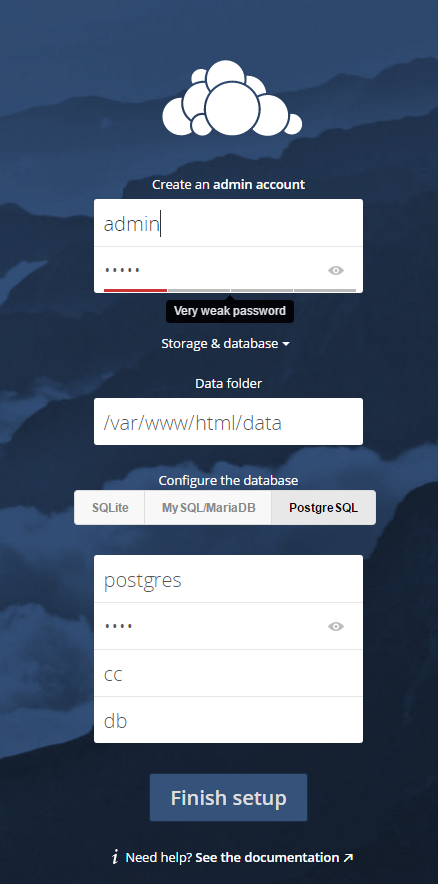
\includegraphics[width=7cm]{img/owncloud-config}
	\caption{Configurando OwnCloud}
	\label{fig:owncloud-config}
\end{figure}

Una vez hecho esto se puede empezar a almacenar ficheros (Figura \ref{fig:owncloud-uploaded-file}):

\begin{figure}[H]
	\centering
	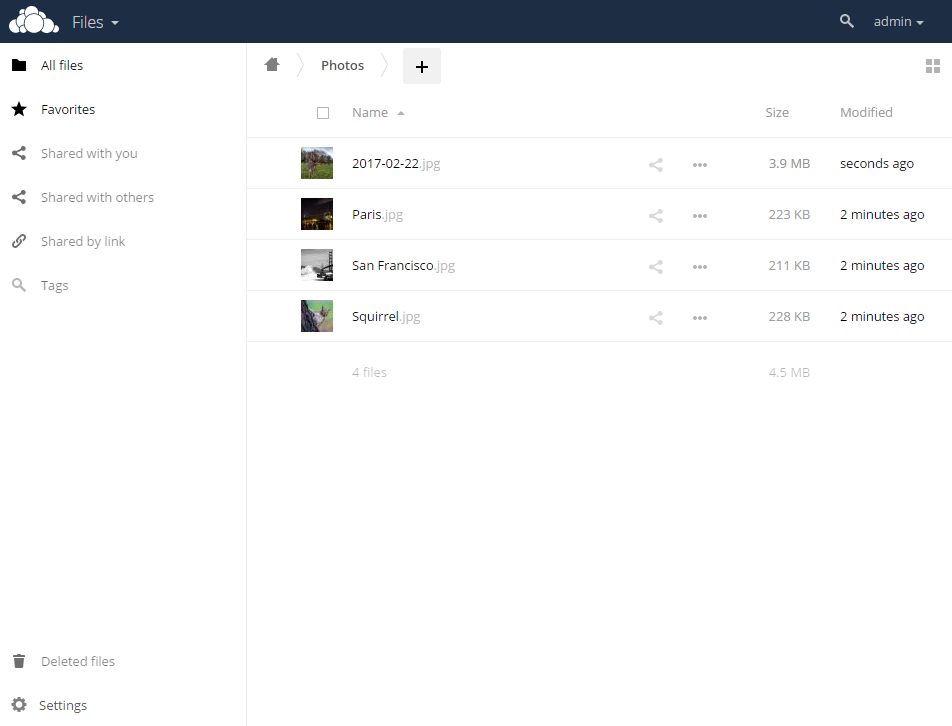
\includegraphics[width=14cm]{img/owncloud-uploaded-file}
	\caption{Imagen subida a OwnCloud con éxito}
	\label{fig:owncloud-uploaded-file}
\end{figure}

\section{Conclusiones}

A diferencia de con OpenNebula, no se han encontrado fallos en la plataforma y se ha podido realizar el trabajo sin problemas.
\\ \\
Además, la práctica en sí es mucho más sencilla que la anterior ya que ya hay contenedores con todo configurado y preparado para empezar a usarse como servidor (web, sistema gestor de base de datos...). Y es que esta es una de las grandes ventajas de los contenedores con respecto a las máquinas virtuales.

%----------------------------------------------------------------------------------------
%	REFERENCIAS
%----------------------------------------------------------------------------------------

\newpage

\bibliography{referencias} %archivo referencias.bib que contiene las entradas 
\bibliographystyle{plain} % hay varias formas de citar

\end{document}